\documentclass[10pt]{article}
\usepackage[a4paper,margin=18mm]{geometry}
\usepackage{amsmath,amssymb,booktabs,array,enumitem,longtable}
\usepackage[T1]{fontenc}\usepackage{lmodern}
\usepackage{tikz}\usetikzlibrary{shapes.gates.logic.US,positioning,arrows.meta,patterns,calc}
\usepackage[hidelinks]{hyperref}
\setlength{\parindent}{0pt}\setlength{\parskip}{4pt}\setlength{\emergencystretch}{2em}
\newcommand{\VDD}{V_{DD}}
\newcommand{\mos}[4]{\begin{scope}[shift={(#1,#2)}]
\draw (0,.24)--(0,-.24);\draw (0,.20)--(.25,.20)--(.25,.5);
\draw (0,-.20)--(.25,-.20)--(.25,-.5);\draw (-.16,.23)--(-.16,-.23);
\ifnum#4=1\draw (-.26,0) circle (.06);\draw (-.75,0)--(-.32,0);\else\draw (-.75,0)--(-.16,0);\fi
\node[anchor=east,font=\scriptsize] at (-.76,0) {$#3$};\end{scope}}
\newcommand{\ground}[2]{\draw (#1,#2)--(#1,{#2-.12});\draw ({#1-.17},{#2-.12})--({#1+.17},{#2-.12});\draw ({#1-.11},{#2-.20})--({#1+.11},{#2-.20});}
\newcommand{\rail}[3]{\draw (#1,#2)--(#1,{#2+.14});\node[above,font=\scriptsize] at (#1,{#2+.14}) {$#3$};}
\newcommand{\hmos}[4]{\begin{scope}[shift={(#1,#2)}]
\draw(-.24,0)--(.24,0);\draw(-.2,0)--(-.2,-.25)--(-.5,-.25);\draw(.2,0)--(.2,-.25)--(.5,-.25);
\draw(-.23,.16)--(.23,.16);
\ifnum#4=1\draw(0,.26)circle(.06);\draw(0,.32)--(0,.75);\else\draw(0,.16)--(0,.75);\fi
\node[below,font=\scriptsize]at(0,-.32){#3};\end{scope}}
\newcommand{\qheading}[1]{\par\medskip\textbf{#1}\par}
\begin{document}
\begin{center}{\large\bfseries Fall 2023 Final: Independently Derived Solutions}\end{center}
The original contains seven questions totaling 115 points. Source bars, clocks, contacts and physical timing paths are retained. The supplied \emph{study compilation} is a mixed-year reference, not a matched graded answer booklet. Numerical conclusions below state their timing and capacitance models.
\qheading{Q1. Short answers (30 points)}
\begin{enumerate}[label=(\alph*),leftmargin=7mm,itemsep=5pt]
\item \textbf{Dynamic power:} signal/load and internal-node charging/discharging, clock-driven switching (clock devices and repeated precharge), and conditional short-circuit overlap current from output inverters, keepers or nonideal clock overlap. An ideal isolated precharge/evaluate core has no unavoidable direct-path overlap. A useful accounting is
\[
P_{dyn}=P_{signal}+P_{clock/precharge}+P_{sc}.
\]
Use disjoint switched-capacitance sets to avoid counting clock or precharge nodes twice. For each set, $P=\alpha C V_{DD}^{2}f$; $\alpha$ counts charging events per cycle. Leakage is static power, rather than a fourth dynamic component.
\item \textbf{Physical design:} turn a circuit/netlist into manufacturable geometry: floorplan, place cells, synthesize the clock distribution, route signal/power nets, and verify the resulting layout.
\item \textbf{Two standard-cell requirements:} compatible cell heights and aligned $V_{DD}/V_{SS}$ rails for row abutment; compliance with the process design rules, including compatible well/implant boundaries and accessible pins. Width may be an integer number of placement sites, rather than equal for every cell.
\item \textbf{Avoid glitches:} balance the arrival times of reconvergent signals, for example by buffering a fast path; restructure or balance logic depth to reduce unequal reconvergent paths. Glitches occur when different path delays temporarily present an unintended input combination. These approaches reduce such events; they do not guarantee zero hazards for arbitrary input changes.
\item \textbf{Two dynamic-logic limitations:} stored-charge nodes can lose noise margin through leakage/charge sharing; directly cascading ordinary same-phase n-type dynamic gates is unsafe because a falling upstream raw output can prematurely discharge the next stage. Domino inserts a static inverter to enforce rising downstream evaluation inputs. Dynamic nodes also require a clock/input protocol.
\item \textbf{Design-rule goal:} impose geometric process constraints so structures can be fabricated with acceptable yield and reliability; for example, minimum widths/spacings and contact enclosure. Rules do not by themselves prove circuit functionality.
\item \textbf{Physical-only cells:} filler cells fill row gaps and preserve well/implant and power-rail continuity; tap cells connect wells/substrates to their bias rails and suppress parasitic latchup; decap cells supply local transient charge and reduce supply noise; endcaps terminate cell-row boundaries with safe well/implant geometry. Cell details depend on the library.
\item \textbf{Two technologies:} a metal-programmable gate array uses prefabricated transistor/base wafers and fewer custom interconnect masks/steps; an FPGA is an already fabricated programmable device, so a new product can avoid a new custom wafer/mask fabrication cycle. The FPGA option shortens product manufacturing lead time by using stocked devices; it does not accelerate the underlying transistor fabrication process. The lecturer also illustrates sea-of-gates, a prefabricated-array variant with custom interconnect. This distinguishes manufacturing lead time from RTL-to-layout design time.
\end{enumerate}
\small Primary course references: Li, Chapters 4 and 6; NCU Digital System Design introduction (gate arrays). Exact URLs and consulted reference-page limitations are recorded in \texttt{sources.json}.\normalsize
\newpage
\qheading{Q2(a). Evaluation and precharge budgets (5 points)}
Let $u=ABC$ and $Y=uD$. Both domino stages receive the \emph{same} clock. Evaluation must allow a three-input output rise followed by a two-input output rise:
\[
t_{eval}\ge3+2=5\ \mathrm{ns}.
\]
Their outputs reset simultaneously during precharge, so
\[
t_{pre}\ge\max(1,1)=1\ \mathrm{ns},
\]
not two serial fall times. Treat the supplied output rise/fall times as the classroom phase budgets. The printed waveform gives no numerical duty cycle.
\begin{center}\begin{tabular}{lll}\toprule
Clock condition&Minimum period&Maximum frequency\\\midrule
Duty adjustable&$5+1=6$ ns&$166.667$ MHz\\
50\% duty&$2\max(5,1)=10$ ns&$100$ MHz\\\bottomrule
\end{tabular}\end{center}
The 6 ns limit uses five-sixths of the cycle for evaluation. The supplied review page 12 explicitly states 50\% duty for a \emph{different} AND--OR exam ($3/2$ ns and $2.5/2$ ns edges). Those premises do not match this AND--AND question ($3/1$ ns and $2/1$ ns); its handwritten annotations have no identifiable grading provenance. Thus no matching graded duty assumption can be inferred, and both conditional results are retained. If these numbers were literal 10--90\% edge times instead of phase-settling budgets, propagation/clock-device timing would need further specification.
\qheading{Q2(b). Retention repair (5 points)}
An unrefreshed dynamic high node can discharge through leakage, so a sufficiently long evaluation interval loses its noise margin. Put a weak pMOS keeper from $V_{DD}$ to each raw n-type dynamic node, with its gate driven by that stage's positive inverter output. The keeper is on for a stored high and turns off after legitimate evaluation discharge. The two-stage implementation below has 15 MOS including two keepers.
\begin{center}\begin{tikzpicture}[x=0.72cm,y=0.72cm,font=\scriptsize]
\mos{0.0}{0.0}{\phi}{1}
\draw(0.25,0.5)--(0.25,0.75)node[above]{$ \mathrm{d1} $};
\draw(0.25,-0.5)--(0.25,-0.75)node[below]{$ V_{DD} $};
\node[anchor=west]at(0.55,0.0){\texttt{PRE1}};
\mos{4.8}{0.0}{A}{0}
\draw(5.05,0.5)--(5.05,0.75)node[above]{$ \mathrm{d1} $};
\draw(5.05,-0.5)--(5.05,-0.75)node[below]{$ \mathrm{s11} $};
\node[anchor=west]at(5.35,0.0){\texttt{N10}};
\mos{9.6}{0.0}{B}{0}
\draw(9.85,0.5)--(9.85,0.75)node[above]{$ \mathrm{s11} $};
\draw(9.85,-0.5)--(9.85,-0.75)node[below]{$ \mathrm{s12} $};
\node[anchor=west]at(10.15,0.0){\texttt{N11}};
\mos{14.399999999999999}{0.0}{C}{0}
\draw(14.649999999999999,0.5)--(14.649999999999999,0.75)node[above]{$ \mathrm{s12} $};
\draw(14.649999999999999,-0.5)--(14.649999999999999,-0.75)node[below]{$ \mathrm{e1} $};
\node[anchor=west]at(14.95,0.0){\texttt{N12}};
\mos{0.0}{-2.8}{\phi}{0}
\draw(0.25,-2.3)--(0.25,-2.05)node[above]{$ \mathrm{e1} $};
\draw(0.25,-3.3)--(0.25,-3.55)node[below]{$ V_{SS} $};
\node[anchor=west]at(0.55,-2.8){\texttt{FOOT1}};
\mos{4.8}{-2.8}{\mathrm{d1}}{1}
\draw(5.05,-2.3)--(5.05,-2.05)node[above]{$ u $};
\draw(5.05,-3.3)--(5.05,-3.55)node[below]{$ V_{DD} $};
\node[anchor=west]at(5.35,-2.8){\texttt{OUT1P}};
\mos{9.6}{-2.8}{\mathrm{d1}}{0}
\draw(9.85,-2.3)--(9.85,-2.05)node[above]{$ u $};
\draw(9.85,-3.3)--(9.85,-3.55)node[below]{$ V_{SS} $};
\node[anchor=west]at(10.15,-2.8){\texttt{OUT1N}};
\mos{14.399999999999999}{-2.8}{u}{1}
\draw(14.649999999999999,-2.3)--(14.649999999999999,-2.05)node[above]{$ \mathrm{d1} $};
\draw(14.649999999999999,-3.3)--(14.649999999999999,-3.55)node[below]{$ V_{DD} $};
\node[anchor=west]at(14.95,-2.8){\texttt{KEEP1} *};
\mos{0.0}{-5.6}{\phi}{1}
\draw(0.25,-5.1)--(0.25,-4.85)node[above]{$ \mathrm{d2} $};
\draw(0.25,-6.1)--(0.25,-6.35)node[below]{$ V_{DD} $};
\node[anchor=west]at(0.55,-5.6){\texttt{PRE2}};
\mos{4.8}{-5.6}{u}{0}
\draw(5.05,-5.1)--(5.05,-4.85)node[above]{$ \mathrm{d2} $};
\draw(5.05,-6.1)--(5.05,-6.35)node[below]{$ \mathrm{s21} $};
\node[anchor=west]at(5.35,-5.6){\texttt{N20}};
\mos{9.6}{-5.6}{D}{0}
\draw(9.85,-5.1)--(9.85,-4.85)node[above]{$ \mathrm{s21} $};
\draw(9.85,-6.1)--(9.85,-6.35)node[below]{$ \mathrm{e2} $};
\node[anchor=west]at(10.15,-5.6){\texttt{N21}};
\mos{14.399999999999999}{-5.6}{\phi}{0}
\draw(14.649999999999999,-5.1)--(14.649999999999999,-4.85)node[above]{$ \mathrm{e2} $};
\draw(14.649999999999999,-6.1)--(14.649999999999999,-6.35)node[below]{$ V_{SS} $};
\node[anchor=west]at(14.95,-5.6){\texttt{FOOT2}};
\mos{0.0}{-8.399999999999999}{\mathrm{d2}}{1}
\draw(0.25,-7.899999999999999)--(0.25,-7.649999999999999)node[above]{$ Y $};
\draw(0.25,-8.899999999999999)--(0.25,-9.149999999999999)node[below]{$ V_{DD} $};
\node[anchor=west]at(0.55,-8.399999999999999){\texttt{OUT2P}};
\mos{4.8}{-8.399999999999999}{\mathrm{d2}}{0}
\draw(5.05,-7.899999999999999)--(5.05,-7.649999999999999)node[above]{$ Y $};
\draw(5.05,-8.899999999999999)--(5.05,-9.149999999999999)node[below]{$ V_{SS} $};
\node[anchor=west]at(5.35,-8.399999999999999){\texttt{OUT2N}};
\mos{9.6}{-8.399999999999999}{Y}{1}
\draw(9.85,-7.899999999999999)--(9.85,-7.649999999999999)node[above]{$ \mathrm{d2} $};
\draw(9.85,-8.899999999999999)--(9.85,-9.149999999999999)node[below]{$ V_{DD} $};
\node[anchor=west]at(10.15,-8.399999999999999){\texttt{KEEP2} *};
\end{tikzpicture}\end{center}
\small Keeper-equipped AND3 followed by AND2; $u$ feeds the second functional nMOS gate. An asterisk marks a weak device. Identically named terminals are connected. All nMOS bodies use $V_{SS}$ and all pMOS bodies use $V_{DD}$.\normalsize\par
Precharge has $\phi=0$: raw nodes $d_1,d_2$ are high and $u,Y$ are low. Evaluation has $\phi=1$: input conditions may discharge a raw node; positive outputs only rise. Keepers must be weak enough to permit discharge and strong enough to overcome leakage. This repair relaxes charge-retention limits while preserving a valid stable/monotone input protocol; it does not justify arbitrary mid-evaluation input changes or an unbounded analog hold time under all conditions.
\newpage
\qheading{Q2(c). Exact input sequence (5 points)}
The original says $(ABCD)=(0000,1110)$, so $D=0$ for \emph{both} patterns. Therefore $Y=uD$ remains 0. For the second evaluation, $u$ rises one delay unit after the clock starts evaluation; precharge makes $u$ fall one unit after the clock falls. One possible phase-aligned waveform is:
\begin{center}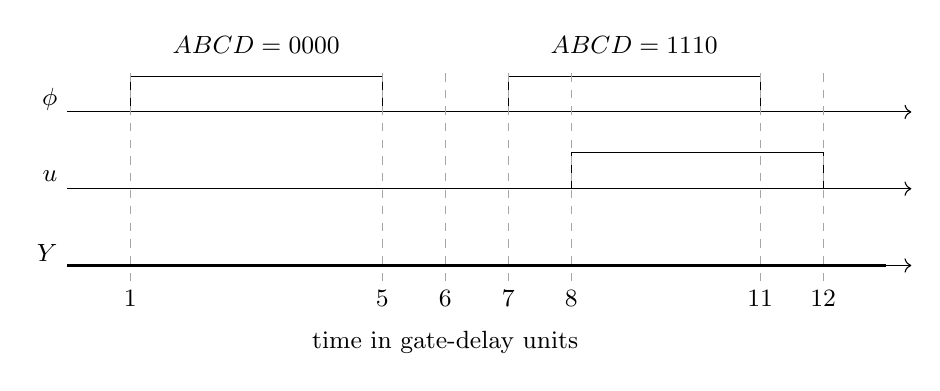
\begin{tikzpicture}[x=.8cm,y=.65cm,font=\small]
\foreach\y/\s in {4/\phi,2.5/u,1/Y}{\draw[->](0,\y)--(13.4,\y);\node[left]at(0,\y+.25){$\s$};}
\draw(0,4)--(1,4)--(1,4.7)--(5,4.7)--(5,4)--(7,4)--(7,4.7)--(11,4.7)--(11,4)--(13,4);
\draw(0,2.5)--(8,2.5)--(8,3.2)--(12,3.2)--(12,2.5)--(13,2.5);
\draw[line width=1pt](0,1)--(13,1);
\foreach\x in {1,5,6,7,8,11,12}{\draw[dashed,black!35](\x,.7)--(\x,4.9);\node[below]at(\x,.7){\x};}
\node at(3,5.3){$ABCD=0000$};\node at(9,5.3){$ABCD=1110$};\node[below]at(6,-.1){time in gate-delay units};
\end{tikzpicture}\end{center}
The input change at unit 6 is during precharge. The phase widths here merely provide slack; they do not assume the Q2(a) nanosecond duty result. The saved waveform CSV lists exact transitions used in this drawing.
\qheading{Q3(a). Read the original clock bars before repairing (5 points)}
Name the unlabeled first raw output $d$, leaving the original internal nodes $x$ and $y$ unchanged. Its pull-down condition is
\[
M=AB+C(A+B),\qquad d=\overline M.
\]
The middle clock is read as $\bar\phi$ in the reconstruction, while the first stage uses $\phi$. Its horizontal stroke touches the footer gate wire in the scan, so this transcription is not claimed to be pixel-unambiguous. Under the opposite-phase reading, when $\phi=0$, $d$ is precharged to 1 and the middle stage evaluates to $\overline Y=0$. When $\phi=1$, the middle stage is forcibly precharged to $\overline Y=1$, independently of $M$: it cycles with the clock rather than providing a usable evaluation-phase function.
If that touching stroke is instead only a wire and the middle clock is $\phi$, direct raw n-dynamic cascading is still unsafe. For example, with $A=B=1,C=0$, the middle can discharge while $d$ is still its precharged 1; when $d$ later falls, the middle cannot recharge during evaluation. This is a valid relative-delay counterexample, rather than a claim that every analog delay ordering gives the same failure.
The right p-type stage is compatible with a raw input falling from 1: it starts at $X=0$ and charges to $X=M$ during $\phi=1$.
\textbf{Primary repair:} make the middle stage a static inverter. Connect its pMOS gate to $d$ and remove its clocked footer, reconnecting the functional nMOS source to $V_{SS}$. This gives $X=M$ and the output \emph{labeled} $\overline Y=M$. The bar is preserved as an output label, rather than used to invent a specified target function.
\newpage
\begin{center}\begin{tikzpicture}[x=0.72cm,y=0.72cm,font=\scriptsize]
\mos{0.0}{0.0}{\phi}{1}
\draw(0.25,0.5)--(0.25,0.75)node[above]{$ d $};
\draw(0.25,-0.5)--(0.25,-0.75)node[below]{$ V_{DD} $};
\node[anchor=west]at(0.55,0.0){\texttt{PRE}};
\mos{4.8}{0.0}{A}{0}
\draw(5.05,0.5)--(5.05,0.75)node[above]{$ d $};
\draw(5.05,-0.5)--(5.05,-0.75)node[below]{$ x $};
\node[anchor=west]at(5.35,0.0){\texttt{A1}};
\mos{9.6}{0.0}{B}{0}
\draw(9.85,0.5)--(9.85,0.75)node[above]{$ x $};
\draw(9.85,-0.5)--(9.85,-0.75)node[below]{$ e $};
\node[anchor=west]at(10.15,0.0){\texttt{B1}};
\mos{14.399999999999999}{0.0}{C}{0}
\draw(14.649999999999999,0.5)--(14.649999999999999,0.75)node[above]{$ d $};
\draw(14.649999999999999,-0.5)--(14.649999999999999,-0.75)node[below]{$ y $};
\node[anchor=west]at(14.95,0.0){\texttt{C1}};
\mos{0.0}{-2.8}{A}{0}
\draw(0.25,-2.3)--(0.25,-2.05)node[above]{$ y $};
\draw(0.25,-3.3)--(0.25,-3.55)node[below]{$ e $};
\node[anchor=west]at(0.55,-2.8){\texttt{A2}};
\mos{4.8}{-2.8}{B}{0}
\draw(5.05,-2.3)--(5.05,-2.05)node[above]{$ y $};
\draw(5.05,-3.3)--(5.05,-3.55)node[below]{$ e $};
\node[anchor=west]at(5.35,-2.8){\texttt{B2}};
\mos{9.6}{-2.8}{\phi}{0}
\draw(9.85,-2.3)--(9.85,-2.05)node[above]{$ e $};
\draw(9.85,-3.3)--(9.85,-3.55)node[below]{$ V_{SS} $};
\node[anchor=west]at(10.15,-2.8){\texttt{FOOT}};
\mos{14.399999999999999}{-2.8}{d}{1}
\draw(14.649999999999999,-2.3)--(14.649999999999999,-2.05)node[above]{$ \overline Y $};
\draw(14.649999999999999,-3.3)--(14.649999999999999,-3.55)node[below]{$ V_{DD} $};
\node[anchor=west]at(14.95,-2.8){\texttt{YMIDP}};
\mos{0.0}{-5.6}{d}{0}
\draw(0.25,-5.1)--(0.25,-4.85)node[above]{$ \overline Y $};
\draw(0.25,-6.1)--(0.25,-6.35)node[below]{$ V_{SS} $};
\node[anchor=west]at(0.55,-5.6){\texttt{YMIDN}};
\mos{4.8}{-5.6}{\bar\phi}{1}
\draw(5.05,-5.1)--(5.05,-4.85)node[above]{$ \mathrm{ex} $};
\draw(5.05,-6.1)--(5.05,-6.35)node[below]{$ V_{DD} $};
\node[anchor=west]at(5.35,-5.6){\texttt{XHEAD}};
\mos{9.6}{-5.6}{d}{1}
\draw(9.85,-5.1)--(9.85,-4.85)node[above]{$ X $};
\draw(9.85,-6.1)--(9.85,-6.35)node[below]{$ \mathrm{ex} $};
\node[anchor=west]at(10.15,-5.6){\texttt{XDATA}};
\mos{14.399999999999999}{-5.6}{\bar\phi}{0}
\draw(14.649999999999999,-5.1)--(14.649999999999999,-4.85)node[above]{$ X $};
\draw(14.649999999999999,-6.1)--(14.649999999999999,-6.35)node[below]{$ V_{SS} $};
\node[anchor=west]at(14.95,-5.6){\texttt{XRESET}};
\end{tikzpicture}\end{center}
\small Q3 primary repair: 12 MOS. The middle pair YMIDP/YMIDN is a static inverter; the first and right stages retain their printed clock phases. Identically named terminals are connected. All nMOS bodies use $V_{SS}$ and all pMOS bodies use $V_{DD}$.\normalsize\par
An alternative valid dynamic repair changes \emph{both} middle clocks to $\phi$ and inserts a static inverter before its functional nMOS. Its positive rising control is $q=\bar d=M$, giving $X=M$ and $\overline Y=\bar M$. This has 15 MOS. The prompt does not specify required output polarities, so both repairs are explicitly identified; they are not presented as the same circuit.
\qheading{Q3(b). Charge sharing with the correctly identified nodes (5 points)}
The supplied node capacitances belong to $x$ (between the series $A,B$ devices) and $y$ (below $C$). They are not a capacitance on $d$. After the primary repair, $d$ sees three diffusion drains (precharge pMOS, top $A$, top $C$), the two middle inverter gates, and one right functional pMOS gate:
\[
C_d^{out}=3C_d+3C_g=0.3+3=3.3\ \mathrm{fF}.
\]
Use the literal supplied \emph{total node parasitic} values $C_x=1.3$ fF and $C_y=1.1$ fF first. If $d$ starts at $V_{DD}$ and a connected internal node starts at 0, charge conservation gives
\[
V_d'=\frac{3.3}{3.3+C_i}V_{DD}.
\]
Non-discharging pattern 100 connects $d$ to $x$, giving $33/46=0.717391$ of $V_{DD}$. Pattern 001 connects it to $y$, giving $3/4=0.75$. Patterns causing $M=1$ intentionally discharge $d$ and are not retention cases. The worst retained voltage exceeds $V_{DD}/2$, so charge sharing alone does not cross the stated switching threshold.
\begin{center}\begin{tabular}{lrrr}\toprule
Interpretation&$C_x$ fF&$C_y$ fF&Worst $V_d'/V_{DD}$\\\midrule
Supplied node values are totals (primary)&1.3&1.1&0.717391\\
Values are wire-only; count every junction&1.5&1.4&0.687500\\
Values are wire-only; count drain terminals only&1.4&1.3&0.702128\\\bottomrule
\end{tabular}\end{center}
The phrase ``parasitic capacitance of the node'' does not explicitly say wire-only. The alternatives show the conclusion is robust without silently double-counting diffusion. Partial precharging of an internal node reduces the drop. This is an ideal charge-conservation/no-leakage check, not an unconditional PVT or long-period correctness claim.
\newpage
\qheading{Q4(1). Dynamic complex gate (15 points shared across three designs)}
To produce the \emph{raw} output $f=\overline{x_1x_2+x_3}$, use an n-type dynamic pull-down network with the $x_1,x_2$ series branch in parallel with $x_3$; add a precharge pMOS and an evaluation footer. Precharge sets $f=1$; evaluation discharges it exactly when $x_1x_2+x_3=1$. Do not add an output inverter and still call its output $f$.
\begin{center}\begin{tikzpicture}[x=0.72cm,y=0.72cm,font=\scriptsize]
\mos{0.0}{0.0}{\phi}{1}
\draw(0.25,0.5)--(0.25,0.75)node[above]{$ f $};
\draw(0.25,-0.5)--(0.25,-0.75)node[below]{$ V_{DD} $};
\node[anchor=west]at(0.55,0.0){\texttt{Ppre}};
\mos{4.8}{0.0}{x_1}{0}
\draw(5.05,0.5)--(5.05,0.75)node[above]{$ f $};
\draw(5.05,-0.5)--(5.05,-0.75)node[below]{$ u $};
\node[anchor=west]at(5.35,0.0){\texttt{Nx1}};
\mos{9.6}{0.0}{x_2}{0}
\draw(9.85,0.5)--(9.85,0.75)node[above]{$ u $};
\draw(9.85,-0.5)--(9.85,-0.75)node[below]{$ e $};
\node[anchor=west]at(10.15,0.0){\texttt{Nx2}};
\mos{14.399999999999999}{0.0}{x_3}{0}
\draw(14.649999999999999,0.5)--(14.649999999999999,0.75)node[above]{$ f $};
\draw(14.649999999999999,-0.5)--(14.649999999999999,-0.75)node[below]{$ e $};
\node[anchor=west]at(14.95,0.0){\texttt{Nx3}};
\mos{0.0}{-2.8}{\phi}{0}
\draw(0.25,-2.3)--(0.25,-2.05)node[above]{$ e $};
\draw(0.25,-3.3)--(0.25,-3.55)node[below]{$ V_{SS} $};
\node[anchor=west]at(0.55,-2.8){\texttt{Nfoot}};
\end{tikzpicture}\end{center}
\small Five-MOS dynamic core. A keeper plus feedback inverter, if required for retention, adds three devices. Identically named terminals are connected. All nMOS bodies use $V_{SS}$ and all pMOS bodies use $V_{DD}$.\normalsize\par
\qheading{Q4(2). Differential pass-transistor logic}
Use Shannon expansion with complementary input rails available:
\[
f=x_1?\bigl(x_2?0:\bar x_3\bigr):\bar x_3,\qquad
g=\bar f=x_1?\bigl(x_2?1:x_3\bigr):x_3.
\]
Four nMOS pass devices realize each rail. Two weak cross-coupled pMOS devices restore the high level, because an nMOS-only pass high otherwise loses a threshold. The differential core therefore has 10 MOS; generating $\bar x_1,\bar x_2,\bar x_3$ locally adds three inverters (six MOS).
\begin{center}\begin{tikzpicture}[x=0.72cm,y=0.72cm,font=\scriptsize]
\mos{0.0}{0.0}{x_1}{0}
\draw(0.25,0.5)--(0.25,0.75)node[above]{$ f $};
\draw(0.25,-0.5)--(0.25,-0.75)node[below]{$ \mathrm{uf} $};
\node[anchor=west]at(0.55,0.0){\texttt{NF1}};
\mos{4.8}{0.0}{\bar x_1}{0}
\draw(5.05,0.5)--(5.05,0.75)node[above]{$ f $};
\draw(5.05,-0.5)--(5.05,-0.75)node[below]{$ \bar x_3 $};
\node[anchor=west]at(5.35,0.0){\texttt{NF0}};
\mos{9.6}{0.0}{x_2}{0}
\draw(9.85,0.5)--(9.85,0.75)node[above]{$ \mathrm{uf} $};
\draw(9.85,-0.5)--(9.85,-0.75)node[below]{$ V_{SS} $};
\node[anchor=west]at(10.15,0.0){\texttt{NF11}};
\mos{14.399999999999999}{0.0}{\bar x_2}{0}
\draw(14.649999999999999,0.5)--(14.649999999999999,0.75)node[above]{$ \mathrm{uf} $};
\draw(14.649999999999999,-0.5)--(14.649999999999999,-0.75)node[below]{$ \bar x_3 $};
\node[anchor=west]at(14.95,0.0){\texttt{NF10}};
\mos{0.0}{-2.8}{x_1}{0}
\draw(0.25,-2.3)--(0.25,-2.05)node[above]{$ g $};
\draw(0.25,-3.3)--(0.25,-3.55)node[below]{$ \mathrm{ug} $};
\node[anchor=west]at(0.55,-2.8){\texttt{NG1}};
\mos{4.8}{-2.8}{\bar x_1}{0}
\draw(5.05,-2.3)--(5.05,-2.05)node[above]{$ g $};
\draw(5.05,-3.3)--(5.05,-3.55)node[below]{$ x_3 $};
\node[anchor=west]at(5.35,-2.8){\texttt{NG0}};
\mos{9.6}{-2.8}{x_2}{0}
\draw(9.85,-2.3)--(9.85,-2.05)node[above]{$ \mathrm{ug} $};
\draw(9.85,-3.3)--(9.85,-3.55)node[below]{$ V_{DD} $};
\node[anchor=west]at(10.15,-2.8){\texttt{NG11}};
\mos{14.399999999999999}{-2.8}{\bar x_2}{0}
\draw(14.649999999999999,-2.3)--(14.649999999999999,-2.05)node[above]{$ \mathrm{ug} $};
\draw(14.649999999999999,-3.3)--(14.649999999999999,-3.55)node[below]{$ x_3 $};
\node[anchor=west]at(14.95,-2.8){\texttt{NG10}};
\mos{0.0}{-5.6}{g}{1}
\draw(0.25,-5.1)--(0.25,-4.85)node[above]{$ f $};
\draw(0.25,-6.1)--(0.25,-6.35)node[below]{$ V_{DD} $};
\node[anchor=west]at(0.55,-5.6){\texttt{PFrestore} *};
\mos{4.8}{-5.6}{f}{1}
\draw(5.05,-5.1)--(5.05,-4.85)node[above]{$ g $};
\draw(5.05,-6.1)--(5.05,-6.35)node[below]{$ V_{DD} $};
\node[anchor=west]at(5.35,-5.6){\texttt{PGrestore} *};
\end{tikzpicture}\end{center}
\small Ten-MOS DPL core. PFrestore gate $g$ and PGrestore gate $f$ are cross-coupled. An asterisk marks a weak device. Identically named terminals are connected. All nMOS bodies use $V_{SS}$ and all pMOS bodies use $V_{DD}$.\normalsize\par
The verifier derives each pass output by source-to-rail graph search, then checks that its level-restoring pair introduces no final rail contention. Analog restorer/pass sizing is not established by an ideal-switch truth table.
\newpage
\qheading{Q4(3). NP-domino XOR}
Preserve all overbars in the original:
\[
f=x_1\oplus x_2=\overline{x_1x_2+\overline{x_1+x_2}}.
\]
First form an n-type raw node $n=\overline{x_1+x_2}$ using two parallel nMOS devices. A p-type second stage has its functional pMOS for $n$ in series with two parallel pMOS devices gated by $x_1,x_2$. It implements
\[
f=\bar n(\bar x_1+\bar x_2)=(x_1+x_2)(\bar x_1+\bar x_2)=x_1\oplus x_2.
\]
For $\phi=0$, $n=1$ and $f=0$. For $\phi=1$, $n$ may only fall, enabling the p-stage to rise. The original primary inputs must be stable during evaluation; the stage-to-stage signal has the required polarity. This circuit requires no complemented primary-input rails.
\begin{center}\begin{tikzpicture}[x=0.72cm,y=0.72cm,font=\scriptsize]
\mos{0.0}{0.0}{\phi}{1}
\draw(0.25,0.5)--(0.25,0.75)node[above]{$ n $};
\draw(0.25,-0.5)--(0.25,-0.75)node[below]{$ V_{DD} $};
\node[anchor=west]at(0.55,0.0){\texttt{NPRE}};
\mos{4.8}{0.0}{x_1}{0}
\draw(5.05,0.5)--(5.05,0.75)node[above]{$ n $};
\draw(5.05,-0.5)--(5.05,-0.75)node[below]{$ \mathrm{en} $};
\node[anchor=west]at(5.35,0.0){\texttt{NX1}};
\mos{9.6}{0.0}{x_2}{0}
\draw(9.85,0.5)--(9.85,0.75)node[above]{$ n $};
\draw(9.85,-0.5)--(9.85,-0.75)node[below]{$ \mathrm{en} $};
\node[anchor=west]at(10.15,0.0){\texttt{NX2}};
\mos{14.399999999999999}{0.0}{\phi}{0}
\draw(14.649999999999999,0.5)--(14.649999999999999,0.75)node[above]{$ \mathrm{en} $};
\draw(14.649999999999999,-0.5)--(14.649999999999999,-0.75)node[below]{$ V_{SS} $};
\node[anchor=west]at(14.95,0.0){\texttt{NFOOT}};
\mos{0.0}{-2.8}{\bar\phi}{1}
\draw(0.25,-2.3)--(0.25,-2.05)node[above]{$ \mathrm{ep} $};
\draw(0.25,-3.3)--(0.25,-3.55)node[below]{$ V_{DD} $};
\node[anchor=west]at(0.55,-2.8){\texttt{PHEAD}};
\mos{4.8}{-2.8}{n}{1}
\draw(5.05,-2.3)--(5.05,-2.05)node[above]{$ \mathrm{ef} $};
\draw(5.05,-3.3)--(5.05,-3.55)node[below]{$ \mathrm{ep} $};
\node[anchor=west]at(5.35,-2.8){\texttt{PN}};
\mos{9.6}{-2.8}{x_1}{1}
\draw(9.85,-2.3)--(9.85,-2.05)node[above]{$ f $};
\draw(9.85,-3.3)--(9.85,-3.55)node[below]{$ \mathrm{ef} $};
\node[anchor=west]at(10.15,-2.8){\texttt{PX1}};
\mos{14.399999999999999}{-2.8}{x_2}{1}
\draw(14.649999999999999,-2.3)--(14.649999999999999,-2.05)node[above]{$ f $};
\draw(14.649999999999999,-3.3)--(14.649999999999999,-3.55)node[below]{$ \mathrm{ef} $};
\node[anchor=west]at(14.95,-2.8){\texttt{PX2}};
\mos{0.0}{-5.6}{\bar\phi}{0}
\draw(0.25,-5.1)--(0.25,-4.85)node[above]{$ f $};
\draw(0.25,-6.1)--(0.25,-6.35)node[below]{$ V_{SS} $};
\node[anchor=west]at(0.55,-5.6){\texttt{PRESET}};
\mos{4.8}{-5.6}{n}{1}
\draw(5.05,-5.1)--(5.05,-4.85)node[above]{$ \bar n $};
\draw(5.05,-6.1)--(5.05,-6.35)node[below]{$ V_{DD} $};
\node[anchor=west]at(5.35,-5.6){\texttt{KNINVP}};
\mos{9.6}{-5.6}{n}{0}
\draw(9.85,-5.1)--(9.85,-4.85)node[above]{$ \bar n $};
\draw(9.85,-6.1)--(9.85,-6.35)node[below]{$ V_{SS} $};
\node[anchor=west]at(10.15,-5.6){\texttt{KNINVN}};
\mos{14.399999999999999}{-5.6}{\bar n}{1}
\draw(14.649999999999999,-5.1)--(14.649999999999999,-4.85)node[above]{$ n $};
\draw(14.649999999999999,-6.1)--(14.649999999999999,-6.35)node[below]{$ V_{DD} $};
\node[anchor=west]at(14.95,-5.6){\texttt{KN} *};
\mos{0.0}{-8.399999999999999}{f}{1}
\draw(0.25,-7.899999999999999)--(0.25,-7.649999999999999)node[above]{$ \bar f $};
\draw(0.25,-8.899999999999999)--(0.25,-9.149999999999999)node[below]{$ V_{DD} $};
\node[anchor=west]at(0.55,-8.399999999999999){\texttt{KFINVP}};
\mos{4.8}{-8.399999999999999}{f}{0}
\draw(5.05,-7.899999999999999)--(5.05,-7.649999999999999)node[above]{$ \bar f $};
\draw(5.05,-8.899999999999999)--(5.05,-9.149999999999999)node[below]{$ V_{SS} $};
\node[anchor=west]at(5.35,-8.399999999999999){\texttt{KFINVN}};
\mos{9.6}{-8.399999999999999}{\bar f}{0}
\draw(9.85,-7.899999999999999)--(9.85,-7.649999999999999)node[above]{$ f $};
\draw(9.85,-8.899999999999999)--(9.85,-9.149999999999999)node[below]{$ V_{SS} $};
\node[anchor=west]at(10.15,-8.399999999999999){\texttt{KF} *};
\end{tikzpicture}\end{center}
\small NP XOR: nine clock/logic MOS plus six keeper/feedback MOS. KN and KF are weak; the feedback inverters supply $\bar n,\bar f$. An asterisk marks a weak device. Identically named terminals are connected. All nMOS bodies use $V_{SS}$ and all pMOS bodies use $V_{DD}$.\normalsize\par
\begin{center}\begin{tabular}{cccccc}\toprule
$x_1$&$x_2$&Evaluation $n$&Evaluation $f$&Precharge $n$&Precharge $f$\\\midrule
0&0&1&0&1&0\\0&1&0&1&1&0\\1&0&0&1&1&0\\1&1&0&0&1&0\\\bottomrule
\end{tabular}\end{center}
Keepers maintain undischarged/uncharged nodes; their transient contention must be sized in a device model. Saved phase checks cover all four inputs in both phases, with exclusive final rail paths.
\newpage
\qheading{Q5(a). Resistance-only classroom sizing (5 points)}
Use the trip points shown by the original waveform: rising-input trip $V_{T+}=1.0$ V and falling-input trip $V_{T-}=0.5$ V. All channel lengths are 40 nm. At fixed length, $R_n\propto1/W_n$ and $R_p\propto2/W_p$ because $\mu_n=2\mu_p$.
\textbf{Fixed external output load $C$:} the falling edge discharges through N2 and N1. Hence
\[
(R_{N1}+R_{N2})C=3RC\quad\Rightarrow\quad R_{N2}=2R,\quad W_{N2}=80\ \mathrm{nm}.
\]
Immediately before the rising-input trip, the lower internal node is $1.0-0.2=0.8$ V. The feedback divider gives
\[
0.8=1.5\frac{R}{R+R_{N3}}\quad\Rightarrow\quad
R_{N3}=\frac78R,\quad W_{N3}=\frac{1280}{7}=182.857\ \mathrm{nm}.
\]
For the falling-input trip, the upper internal node is $0.5+0.2=0.7$ V:
\[
0.7=1.5\frac{R_{P3}}{R_{P1}+R_{P3}}\quad\Rightarrow\quad R_{P3}=\frac78R_{P1}.
\]
The rising edge requires $R_{P1}+R_{P2}=3R$. These equations do not uniquely determine the pMOS pair. With $a=R_{P1}/R$, the family is
\[
0<a<3,\quad W_{P1}=\frac{320}{a},\quad W_{P2}=\frac{320}{3-a},\quad
W_{P3}=\frac{2560}{7a}\quad(\mathrm{nm}).
\]
Choose $a=1$ (P1 has the resistance of N1) to give one explicit valid classroom design:
\begin{center}\begin{tabular}{lrr}\toprule
Device&Width nm&Length nm\\\midrule
N1 (given)&160&40\\N2&80&40\\N3&182.857&40\\P1&320&40\\P2&160&40\\P3&365.714&40\\\bottomrule
\end{tabular}\end{center}
The matched-resistance choice is stated as an additional selection, not a hidden condition in the original.
\qheading{Literal feedback-gate capacitance reading: infeasible}
The output physically also drives N3 and P3 gates. If their gate capacitances are included, with $C\propto W$ and the explicit load equal to the N1 gate capacitance,
\[
K=\frac{C_{out}}{C}=1+\frac{W_{N3}+W_{P3}}{160}=\frac{15}{7}+\frac{16}{7a}.
\]
Positive N2 resistance requires $(1+R_{N2}/R)K=3$, so $K<3$, implying $a>8/3$. Positive P2 resistance requires $(a+R_{P2}/R)K=3$, so $aK<3$, implying $a<1/3$. These conditions contradict each other. Thus no positive finite device widths satisfy the specified 3RC edges under that literal gate-capacitance model, even with drain caps neglected. The geometry table applies to the fixed-$C$ classroom model only.
\newpage
\qheading{Q5(b). Turning on the added feedback devices (10 points)}
Enabling the switches connects the added N4/P4 gates to the output and puts their channels in parallel with N3/P3. The effective feedback resistances decrease, strengthening positive feedback. The upper trip rises and the lower trip falls; the hysteresis window and tolerance of excursions inside that window increase.
For an illustrative explicit case $N4=N3$ and $P4=P3$, each feedback resistance halves. For the $a=1$ sizing above,
\[
V_{T+}^{on}=1.5\frac{R}{R+7R/16}+0.2=1.243478\ \mathrm V,
\]
\[
V_{T-}^{on}=1.5\frac{7R/16}{R+7R/16}-0.2=0.256522\ \mathrm V.
\]
The window increases from $1.0-0.5=0.5$ V to $0.986957$ V. The original does not specify N4/P4 widths, so these new numerical thresholds are an example, not uniquely required values.
The resistance-only classroom conclusion for short-circuit power is \textbf{increased}: enabling a parallel feedback path lowers the resistance of the feedback supply-to-ground overlap path at a given input bias. A numerical or universally monotone \emph{cycle-average} $P_{sc}$ cannot be obtained from the supplied data alone: hysteresis also changes when the output transitions, and integrated overlap current depends on input slew, period, added sizes and transistor characteristics. No peak or edge-average is mislabeled as a cycle-average result.
\qheading{Q6. Extract all seven poly crossings per active row (10 points)}
Reading contacts rather than judging a low-resolution silhouette gives the following active-segment nets, left to right:
\begin{center}\begin{tabular}{lll}\toprule
Row&Eight successive active segments&Seven successive poly gates\\\midrule
pMOS&$V_{DD},x,V_{DD},p_1,p_2,w,V_{DD},z$&$a,V_{DD},x,b,c,V_{DD},w$\\
nMOS&$V_{SS},x,V_{SS},w,V_{SS},w,V_{SS},z$&$a,V_{SS},x,b,c,V_{SS},w$\\\bottomrule
\end{tabular}\end{center}
There are \textbf{14 physical MOS}. Columns 2 and 6 are split isolation gates tied to $V_{DD}$ in the p-row and $V_{SS}$ in the n-row; all four devices are off. The other ten devices implement
\[
x=\bar a,\qquad w=\overline{x+b+c},\qquad z=\bar w=\bar a+b+c.
\]
The top $p_1,p_2$ local contact/metal patches are series-node islands, not power contacts. A metal crossing over poly without a black contact square is insulated. The middle $w$ metal strap joins the relevant n-active segments and drives the final inverter gate; it crosses the $b,c$ polys without shorting their gates. The physical transistor schematic on the next page preserves the four isolation devices rather than deleting them from the source extraction.
\newpage
\begin{center}\begin{tikzpicture}[x=0.72cm,y=0.72cm,font=\scriptsize]
\mos{0.0}{0.0}{a}{1}
\draw(0.25,0.5)--(0.25,0.75)node[above]{$ x $};
\draw(0.25,-0.5)--(0.25,-0.75)node[below]{$ V_{DD} $};
\node[anchor=west]at(0.55,0.0){\texttt{P1}};
\mos{4.8}{0.0}{V_{DD}}{1}
\draw(5.05,0.5)--(5.05,0.75)node[above]{$ V_{DD} $};
\draw(5.05,-0.5)--(5.05,-0.75)node[below]{$ x $};
\node[anchor=west]at(5.35,0.0){\texttt{P2}};
\mos{9.6}{0.0}{x}{1}
\draw(9.85,0.5)--(9.85,0.75)node[above]{$ \mathrm{p1} $};
\draw(9.85,-0.5)--(9.85,-0.75)node[below]{$ V_{DD} $};
\node[anchor=west]at(10.15,0.0){\texttt{P3}};
\mos{14.399999999999999}{0.0}{b}{1}
\draw(14.649999999999999,0.5)--(14.649999999999999,0.75)node[above]{$ \mathrm{p2} $};
\draw(14.649999999999999,-0.5)--(14.649999999999999,-0.75)node[below]{$ \mathrm{p1} $};
\node[anchor=west]at(14.95,0.0){\texttt{P4}};
\mos{0.0}{-2.8}{c}{1}
\draw(0.25,-2.3)--(0.25,-2.05)node[above]{$ w $};
\draw(0.25,-3.3)--(0.25,-3.55)node[below]{$ \mathrm{p2} $};
\node[anchor=west]at(0.55,-2.8){\texttt{P5}};
\mos{4.8}{-2.8}{V_{DD}}{1}
\draw(5.05,-2.3)--(5.05,-2.05)node[above]{$ V_{DD} $};
\draw(5.05,-3.3)--(5.05,-3.55)node[below]{$ w $};
\node[anchor=west]at(5.35,-2.8){\texttt{P6}};
\mos{9.6}{-2.8}{w}{1}
\draw(9.85,-2.3)--(9.85,-2.05)node[above]{$ z $};
\draw(9.85,-3.3)--(9.85,-3.55)node[below]{$ V_{DD} $};
\node[anchor=west]at(10.15,-2.8){\texttt{P7}};
\mos{14.399999999999999}{-2.8}{a}{0}
\draw(14.649999999999999,-2.3)--(14.649999999999999,-2.05)node[above]{$ x $};
\draw(14.649999999999999,-3.3)--(14.649999999999999,-3.55)node[below]{$ V_{SS} $};
\node[anchor=west]at(14.95,-2.8){\texttt{N1}};
\mos{0.0}{-5.6}{V_{SS}}{0}
\draw(0.25,-5.1)--(0.25,-4.85)node[above]{$ V_{SS} $};
\draw(0.25,-6.1)--(0.25,-6.35)node[below]{$ x $};
\node[anchor=west]at(0.55,-5.6){\texttt{N2}};
\mos{4.8}{-5.6}{x}{0}
\draw(5.05,-5.1)--(5.05,-4.85)node[above]{$ w $};
\draw(5.05,-6.1)--(5.05,-6.35)node[below]{$ V_{SS} $};
\node[anchor=west]at(5.35,-5.6){\texttt{N3}};
\mos{9.6}{-5.6}{b}{0}
\draw(9.85,-5.1)--(9.85,-4.85)node[above]{$ V_{SS} $};
\draw(9.85,-6.1)--(9.85,-6.35)node[below]{$ w $};
\node[anchor=west]at(10.15,-5.6){\texttt{N4}};
\mos{14.399999999999999}{-5.6}{c}{0}
\draw(14.649999999999999,-5.1)--(14.649999999999999,-4.85)node[above]{$ w $};
\draw(14.649999999999999,-6.1)--(14.649999999999999,-6.35)node[below]{$ V_{SS} $};
\node[anchor=west]at(14.95,-5.6){\texttt{N5}};
\mos{0.0}{-8.399999999999999}{V_{SS}}{0}
\draw(0.25,-7.899999999999999)--(0.25,-7.649999999999999)node[above]{$ V_{SS} $};
\draw(0.25,-8.899999999999999)--(0.25,-9.149999999999999)node[below]{$ w $};
\node[anchor=west]at(0.55,-8.399999999999999){\texttt{N6}};
\mos{4.8}{-8.399999999999999}{w}{0}
\draw(5.05,-7.899999999999999)--(5.05,-7.649999999999999)node[above]{$ z $};
\draw(5.05,-8.899999999999999)--(5.05,-9.149999999999999)node[below]{$ V_{SS} $};
\node[anchor=west]at(5.35,-8.399999999999999){\texttt{N7}};
\end{tikzpicture}\end{center}
\small Q6 full physical schematic: P1--P7 and N1--N7 follow the seven columns left to right; P2/N2/P6/N6 are rail-tied off isolation devices. Identically named terminals are connected. All nMOS bodies use $V_{SS}$ and all pMOS bodies use $V_{DD}$.\normalsize\par
\begin{center}\begin{tabular}{cccccc}\toprule
$a$&$b$&$c$&$x$&$w$&$z$\\\midrule
0&0&0&1&0&1\\0&0&1&1&0&1\\0&1&0&1&0&1\\0&1&1&1&0&1\\
1&0&0&0&1&0\\1&0&1&0&0&1\\1&1&0&0&0&1\\1&1&1&0&0&1\\\bottomrule
\end{tabular}\end{center}
The checker obtains $x,w,z$ by finding conducting rail paths stage by stage, verifies both rail exclusivity and the independently derived function, and exports every device's gate/active/body net in \texttt{q6\_physical\_MOS.csv}.
\qheading{Q7. Preserve the printed reconvergent path}
Let $q_i=R_i.Q$ and $v=q_2q_3q_4$. The printed graph is
\[
R5.D=q_1,\quad R6.D=\overline{q_1+v},\quad R7.D=v,\quad
R8.D=\overline{\bar v+q_4}=v\bar q_4=0.
\]
The last Boolean simplification does not authorize removing the original physical gates when answering the timing question. The R8 reconvergent path may glitch and must settle before its capture edge. No connection is silently changed to create a different conventional circuit.
For a concrete hazard, start $q_2=q_3=q_4=1$ and let $q_4$ fall after the 0.2 ns clock-to-Q delay. The direct NOR input falls at 0.2 ns, but $\bar v$ rises only at $0.2+0.5+0.5+0.2=1.4$ ns. With the final 0.5 ns NOR delay, R8.D rises at 0.7 ns and settles low at 1.9 ns. The saved event CSV records this valid pulse under the printed delay model.
\newpage
\qheading{Q7(a). Hold failure and lockup latch (5 points)}
At zero skew the direct R1--R5 path has no logic delay. New data can arrive after $t_{ccq}=0.1$ ns, while R5 must hold for 0.2 ns: $0.1<0.2$, a 0.1 ns hold violation. Increasing the period cannot repair this direct same-edge hold violation.
Insert a \textbf{low-level transparent lockup latch} only on the R1-to-R5 data branch. It closes at the launching positive edge, holds the old data during the high clock phase, and opens at the falling edge. The R1 branch to R6 remains direct. The latch uses the launch clock; its own timing limits must be satisfied.
\begin{center}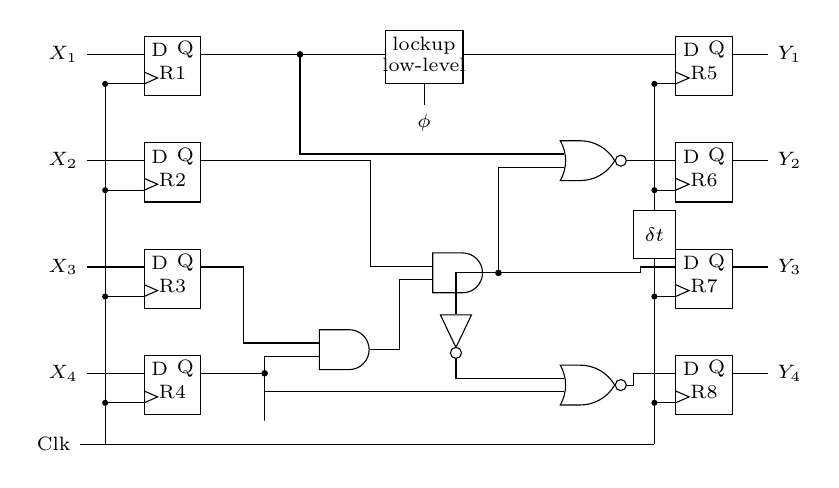
\begin{tikzpicture}[x=.9cm,y=.75cm,font=\scriptsize]
\draw(0.29999999999999993,6.5)rectangle(1.1,7.5);\node at(0.7,6.88){R1};
\node at(0.52,7.27){D};\node at(0.8799999999999999,7.27){Q};
\draw(0.29999999999999993,6.7)--(0.49,6.8)--(0.29999999999999993,6.9);
\draw(7.799999999999999,6.5)rectangle(8.6,7.5);\node at(8.2,6.88){R5};
\node at(8.02,7.27){D};\node at(8.379999999999999,7.27){Q};
\draw(7.799999999999999,6.7)--(7.989999999999999,6.8)--(7.799999999999999,6.9);
\draw(-.5,7.2)--(.3,7.2)node[pos=0,left]{$X_1$};
\draw(8.6,7.2)--(9.1,7.2)node[right]{$Y_1$};
\draw(0.29999999999999993,4.7)rectangle(1.1,5.7);\node at(0.7,5.08){R2};
\node at(0.52,5.470000000000001){D};\node at(0.8799999999999999,5.470000000000001){Q};
\draw(0.29999999999999993,4.9)--(0.49,5.0)--(0.29999999999999993,5.1000000000000005);
\draw(7.799999999999999,4.7)rectangle(8.6,5.7);\node at(8.2,5.08){R6};
\node at(8.02,5.470000000000001){D};\node at(8.379999999999999,5.470000000000001){Q};
\draw(7.799999999999999,4.9)--(7.989999999999999,5.0)--(7.799999999999999,5.1000000000000005);
\draw(-.5,5.4)--(.3,5.4)node[pos=0,left]{$X_2$};
\draw(8.6,5.4)--(9.1,5.4)node[right]{$Y_2$};
\draw(0.29999999999999993,2.9)rectangle(1.1,3.9);\node at(0.7,3.28){R3};
\node at(0.52,3.67){D};\node at(0.8799999999999999,3.67){Q};
\draw(0.29999999999999993,3.1)--(0.49,3.1999999999999997)--(0.29999999999999993,3.3);
\draw(7.799999999999999,2.9)rectangle(8.6,3.9);\node at(8.2,3.28){R7};
\node at(8.02,3.67){D};\node at(8.379999999999999,3.67){Q};
\draw(7.799999999999999,3.1)--(7.989999999999999,3.1999999999999997)--(7.799999999999999,3.3);
\draw(-.5,3.6)--(.3,3.6)node[pos=0,left]{$X_3$};
\draw(8.6,3.6)--(9.1,3.6)node[right]{$Y_3$};
\draw(0.29999999999999993,1.0999999999999996)rectangle(1.1,2.0999999999999996);\node at(0.7,1.4799999999999995){R4};
\node at(0.52,1.8699999999999997){D};\node at(0.8799999999999999,1.8699999999999997){Q};
\draw(0.29999999999999993,1.2999999999999996)--(0.49,1.3999999999999997)--(0.29999999999999993,1.4999999999999996);
\draw(7.799999999999999,1.0999999999999996)rectangle(8.6,2.0999999999999996);\node at(8.2,1.4799999999999995){R8};
\node at(8.02,1.8699999999999997){D};\node at(8.379999999999999,1.8699999999999997){Q};
\draw(7.799999999999999,1.2999999999999996)--(7.989999999999999,1.3999999999999997)--(7.799999999999999,1.4999999999999996);
\draw(-.5,1.7999999999999996)--(.3,1.7999999999999996)node[pos=0,left]{$X_4$};
\draw(8.6,1.7999999999999996)--(9.1,1.7999999999999996)node[right]{$Y_4$};
\node[and gate US,draw,logic gate inputs=nn] (a1) at(3.1,2.2) {};
\node[and gate US,draw,logic gate inputs=nn] (a2) at(4.7,3.5) {};
\node[nor gate US,draw,logic gate inputs=nn] (n1) at(6.5,5.4) {};
\node[nor gate US,draw,logic gate inputs=nn] (n2) at(6.5,1.6) {};
\node[not gate US,draw,rotate=-90] (iv) at(4.7,2.6) {};
\draw(1.1,3.6)--(1.7,3.6)|-(a1.input 1);
\draw(1.1,1.8)--(2,1.8)|-(a1.input 2);
\draw(1.1,5.4)--(3.5,5.4)|-(a2.input 1);\draw(a1.output)--(3.9,2.2)|-(a2.input 2);
\draw(a2.output)--(5.3,3.5)--(7.3,3.5)|-(7.8,3.6);\fill(5.3,3.5)circle(1.2pt);
\draw(5.3,3.5)--(5.3,5.1)|-(n1.input 2);\draw(5.3,3.5)--(4.7,3.5)--(iv.input);
\draw(iv.output)--(4.7,1.8)|-(n2.input 1);
\draw(2,1.8)--(2,1)|-(n2.input 2);\fill(2,1.8)circle(1.2pt);
\draw(n1.output)--(7.8,5.4);\draw(n2.output)--(7.2,1.6)|-(7.8,1.8);
\draw(1.1,7.2)--(3.7,7.2);\draw(3.7,6.7)rectangle(4.8,7.6);\node at(4.25,7.35){lockup};\node at(4.25,7.02){low-level};\draw(4.8,7.2)--(7.8,7.2);
\draw(4.25,6.7)--(4.25,6.35)node[below]{$\phi$};
\draw(2.5,7.2)--(2.5,6)|-(n1.input 1);\fill(2.5,7.2)circle(1.2pt);
\draw(-.25,.6)--(-.25,6.7);\draw(-.6,.6)--(7.5,.6)node[pos=0,left]{Clk};
\draw(-.25,6.7)--(.3,6.7);\fill(-.25,6.7)circle(1.1pt);
\draw(7.5,6.7)--(7.8,6.7);\fill(7.5,6.7)circle(1.1pt);
\draw(-.25,4.9)--(.3,4.9);\fill(-.25,4.9)circle(1.1pt);
\draw(7.5,4.9)--(7.8,4.9);\fill(7.5,4.9)circle(1.1pt);
\draw(-.25,3.1)--(.3,3.1);\fill(-.25,3.1)circle(1.1pt);
\draw(7.5,3.1)--(7.8,3.1);\fill(7.5,3.1)circle(1.1pt);
\draw(-.25,1.3)--(.3,1.3);\fill(-.25,1.3)circle(1.1pt);
\draw(7.5,1.3)--(7.8,1.3);\fill(7.5,1.3)circle(1.1pt);
\draw(7.5,.6)--(7.5,3.75);\draw(7.5,4.55)--(7.5,6.7);
\draw(7.2,3.75)rectangle(7.8,4.55);\node at(7.5,4.15){$\delta t$};
\end{tikzpicture}\end{center}
\begin{center}\small Q7(a) repair: A sequential circuit. The inline capture-clock delay is below R6 and above R7.\end{center}
The capture clock stem places $\delta t$ \emph{between} the R7 and R6 taps. Thus a positive delay shifts R5 and R6 capture clocks later; R7 and R8 remain undelayed.
\qheading{Q7(b). Propagation bound at $\delta t=0$ (5 points)}
The longest original physical logic path is R3/R4--AND--AND--INV--NOR--R8:
\[
t_{logic,max}=0.5+0.5+0.2+0.5=1.7\ \mathrm{ns}.
\]
Ignoring wire delay as instructed, the register setup condition gives
\[
T\ge t_{pcq}+t_{logic,max}+t_{setup}=0.2+1.7+0.2=2.1\ \mathrm{ns}.
\]
\textbf{Conditional ideal-latch result:} $f_{max}=1/(2.1\,\mathrm{ns})=476.190$ MHz if the inserted latch and all actual minimum-delay paths satisfy the conditions on the next page. The original does not give latch propagation/setup/hold parameters, so this is not an unconditional implementation guarantee.
\newpage
\qheading{Q7(b,c). Missing latch parameters and positive skew (10 points combined)}
Write $t_{pd,L},t_{cd,L},t_{hold,L},t_{setup,L}$ for the latch properties. Let the unspecified high phase last $H$; the latch opens at $H$. Provided $H\ge0.2$ ns, general bounds are $T+\delta t-H\ge t_{pd,L}+0.2$ ns for setup and $H+t_{cd,L}\ge\delta t+0.2$ ns for hold. For an explicitly selected 50\% clock, $H=T/2$ and setup at R5 requires
\[
T/2+\delta t\ge t_{pd,L}+0.2\ \mathrm{ns};
\]
hold at R5 requires its earliest released new data to satisfy
\[
T/2+t_{cd,L}\ge\delta t+0.2\ \mathrm{ns}.
\]
At the coincident launch edge/latch closing edge, the latch's own hold condition additionally needs $t_{hold,L}\le0.1$ ns. The preceding old-data setup condition must also be met (a sufficient steady-cycle bound is $t_{setup,L}\le T-0.2$ ns); no latch setup number is invented.
\begin{center}\begin{tabular}{lrr}\toprule
At $T=2.1$ ns&$\delta t=0$&$\delta t=0.3$ ns\\\midrule
Allowed $t_{pd,L}$ upper bound&0.85 ns&1.15 ns\\
Required $t_{cd,L}$ lower bound&0 ns&0 ns\\
R5 hold margin with $t_{cd,L}=0$&0.85 ns&0.55 ns\\
Latch's own allowed hold&$\le0.1$ ns&$\le0.1$ ns\\\bottomrule
\end{tabular}\end{center}
For any ordinary register-to-register path, with capture skew $s$ relative to launch,
\[
T\ge0.2+t_{logic,prop}+0.2-s,\qquad
t_{logic,cont}\ge s+0.2-0.1=s+0.1.
\]
The printed gate ``delays'' provide propagation numbers, but no separate contamination delays. If the classroom convention treats those numbers as both minimum and maximum, the remaining paths satisfy hold for both skews (the shortest affected R6 path is 0.5 ns, exceeding 0.4 ns). In a real timing model, verify these minimum-delay bounds separately; propagation delay alone cannot prove hold.
\begin{center}\begin{tabular}{llrr}\toprule
Representative path&Logic ns&Setup $T$ at skew0&Setup $T$ at $\delta t=.3$\\\midrule
R1--NOR--R6&0.5&0.9&0.6\\
R3/R4--AND--AND--NOR--R6&1.5&1.9&1.6\\
R3/R4--AND--AND--R7&1.0&1.4&1.4\\
R3/R4--AND--AND--INV--NOR--R8&1.7&2.1&2.1\\\bottomrule
\end{tabular}\end{center}
For $\delta t=0.3$ ns the \emph{unmodified} direct R1--R5 path is still invalid: $0.1<0.3+0.2=0.5$ ns. The latch-repaired circuit remains valid under the stated latch/minimum-delay bounds, and R8 retains the same 2.1 ns setup limit. Thus its conditional ideal-latch maximum frequency stays \textbf{476.190 MHz}.
\newpage
\qheading{Q7(d). Clock distribution (5 points)}
The lecturer's Chapter 7 names \textbf{H-tree} and \textbf{balanced-tree} distribution as the two most common physical clocking networks.
An H-tree splits into symmetric branches with equal root-to-leaf geometric path lengths; matched wire geometry and balanced buffers/loading reduce arrival differences. For irregular register positions, the leaves feed local balanced trees rather than requiring registers to lie on a perfect geometric grid.
A balanced tree groups sinks and adjusts wire lengths, buffers and loads to equalize \emph{electrical} root-to-sink delay. Equalized RC/buffer delays reduce skew even with irregular sink placement. Physical symmetry alone is insufficient if load or wire geometry differs. A clock mesh is another valid option: connected paths average local delay variation, at the cost of more wire/clock power, but it is not needed to replace the lecturer's expected pair here.
\begin{center}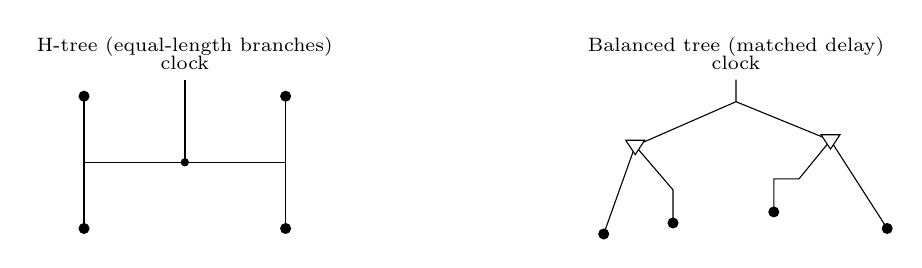
\begin{tikzpicture}[x=.8cm,y=.7cm,font=\scriptsize]
\node at(2,3.6){H-tree (equal-length branches)};
\draw[line width=.8pt](2,3)--(2,1.5);\draw(.4,1.5)--(3.6,1.5);
\draw(.4,.3)--(.4,2.7);\draw(3.6,.3)--(3.6,2.7);
\foreach\x/\y in {.4/.3,.4/2.7,3.6/.3,3.6/2.7}{\fill(\x,\y)circle(2pt);}
\fill(2,1.5)circle(1.5pt);
\node[above]at(2,3){clock};
\begin{scope}[xshift=7cm]
\node at(2,3.6){Balanced tree (matched delay)};
\draw(2,3)--(2,2.6)--(.4,1.8);\draw(2,2.6)--(3.5,1.9);
\draw(.4,1.8)--(-.1,.2);\draw(.4,1.8)--(1,1)--(1,.4);
\draw(3.5,1.9)--(3,1.2)--(2.6,1.2)--(2.6,.6);\draw(3.5,1.9)--(4.4,.3);
\foreach\x/\y in {-.1/.2,1/.4,2.6/.6,4.4/.3}{\fill(\x,\y)circle(2pt);}
\foreach\x/\y in {.4/1.8,3.5/1.9}{\draw[fill=white](\x-.15,\y+.1)--(\x+.15,\y+.1)--(\x,\y-.16)--cycle;}
\node[above]at(2,3){clock};\end{scope}
\end{tikzpicture}\end{center}
\qheading{Reference comparison and reproducibility}
The original exam is the two-page Fall 2023 printed source. The supplied \emph{Final Review} reference has 17 pages of mixed-year study material; it is not identified as a graded solution to this complete paper. Its common-cell and dynamic-logic notes are useful background. Its other clock, Schmitt and logic questions have different diagrams/parameters and are not evidence for 2023 numerical answers.
The final solutions derive clocks, transistor edges, bars, trip thresholds and timing independently. In particular: Q2 uses the actual 1110 second input; Q3 records the touching clock-stroke ambiguity and correctly locates internal-node $x$; Q5 declares its extra resistance/capacitance assumptions; Q6 preserves 14 physical devices; Q7 preserves the constant-output reconvergent physical path and the correct delayed clock taps.
Run \texttt{python verify\_logic\_timing.py}. It regenerates the saved CSVs and \texttt{logic\_timing\_verification.json} using only the Python standard library. These are exhaustive ideal-switch/logic and analytical timing/charge checks, not HSPICE measurements. The PDF needs no external figures; all drawings are inline TikZ.
\qheading{Primary references}
{\raggedright
\begin{enumerate}[leftmargin=6mm,itemsep=3pt]
\item Li, NCU, VLSI Chapter 4 (glitch power), slides 58--67: \url{https://staff.ee.ncu.edu.tw/jfli/public_html/VLSI/lecture/ch04.pdf}.
\item Li, NCU, VLSI Chapter 6 (dynamic logic): \url{https://www.ee.ncu.edu.tw/jfli/public_html/VLSI/lecture/ch06.pdf}.
\item Li, NCU, VLSI Chapter 7, clock distribution slide 37: \url{https://www.ee.ncu.edu.tw/jfli/public_html/VLSI/lecture/ch07.pdf}.
\item NCU, Digital System Design introduction (gate arrays): \url{https://www.ee.ncu.edu.tw/jimmy/public_html/courses/DSD06/01_intro.pdf}.
\item Li, NCU, VLSI Chapter 5 (physical design/arrays), slides 3--31: \url{https://www.ee.ncu.edu.tw/jfli/public_html/VLSI/lecture/ch05.pdf}.
\item Cadence physical-only cell training: \url{https://community.cadence.com/cadence_blogs_8/b/di/posts/you-know-how-but-do-you-remember-why}.
\item Georgia Tech author-hosted IEEE tap/latchup study, printed page 1728: \url{https://gtcad.gatech.edu/www/papers/06423265.pdf}.
\item David Harris, Harvey Mudd, cell design lecture, slides 8--14: \url{https://pages.hmc.edu/harris/class/e158/01/lect09.pdf}.
\end{enumerate}
\par}
\end{document}
